

% \chapter{Reproducibility self-assessment}

% \section{Marks for each of the criteria}

% \begin{figure}[h]
%   \centering
%   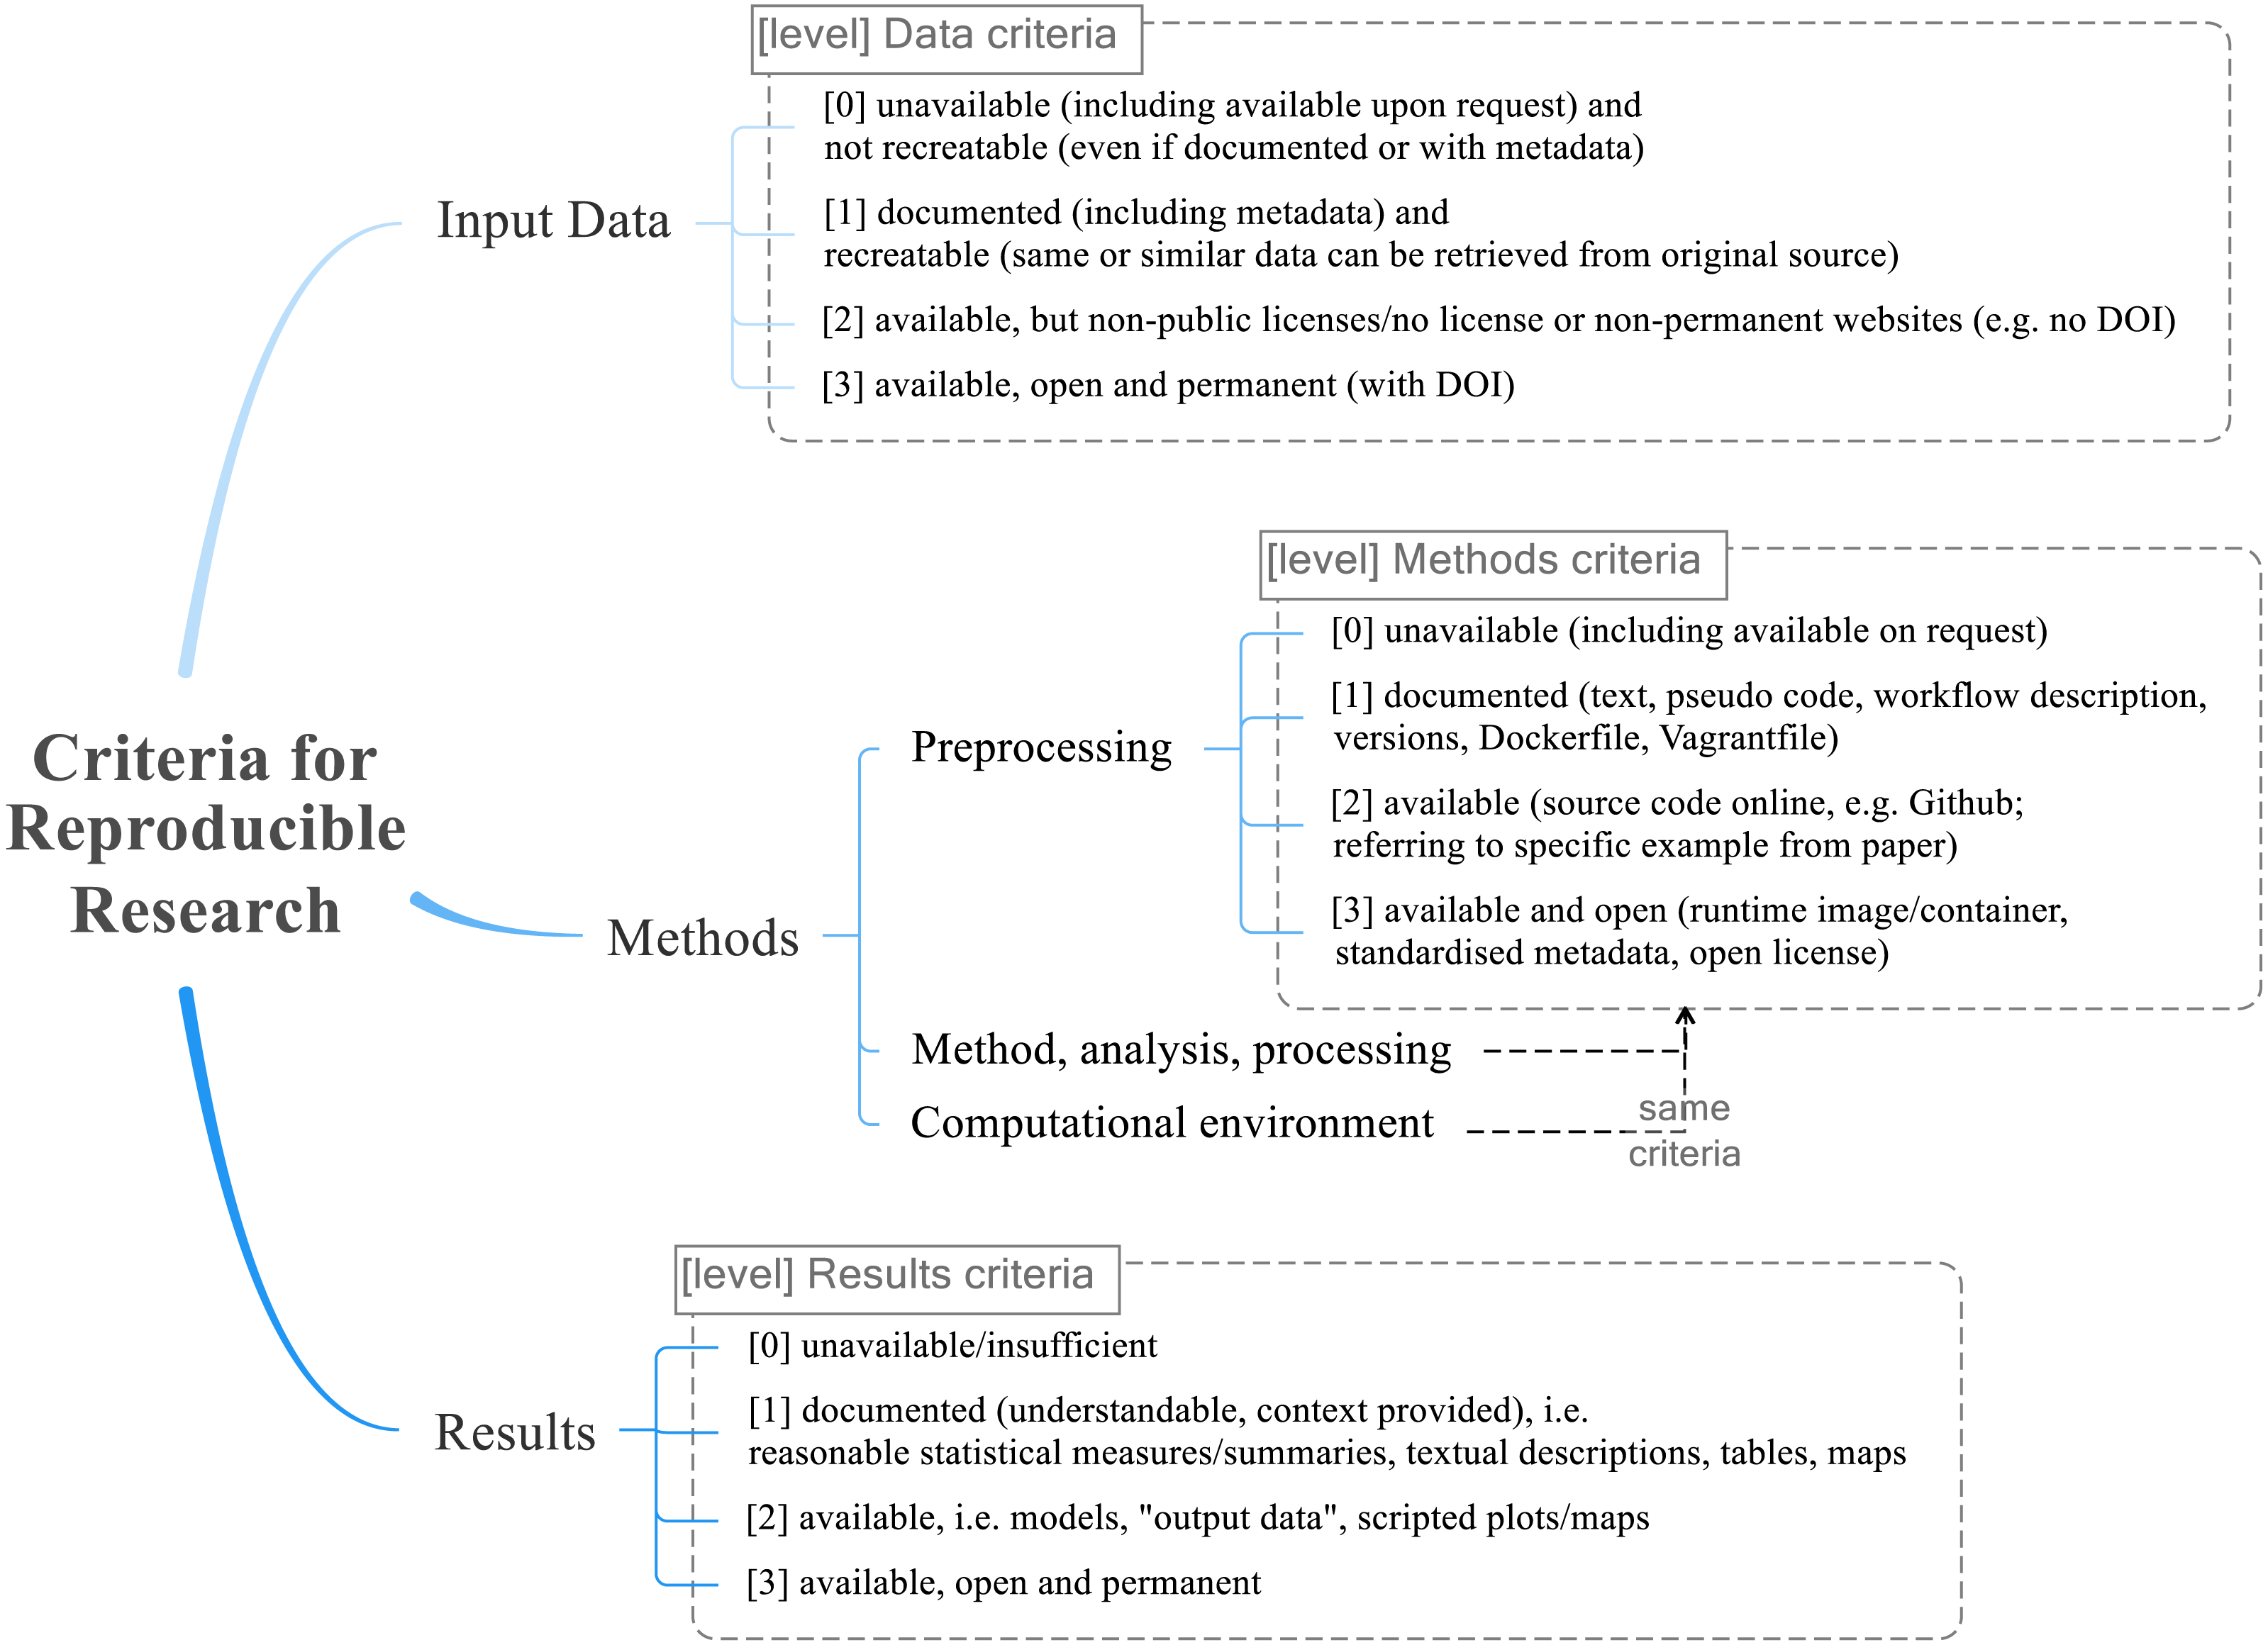
\includegraphics[width=0.8\linewidth]{figs/reproducibility_criteria.png}
%   \caption{Reproducibility criteria to be assessed.}
% \label{fig:reproducibility_criteria}
% \end{figure}

% Grade/evaluate yourself for the 5 criteria (giving 0/1/2/3 for each):
% \begin{enumerate}
%   \item input data
%   \item preprocessing
%   \item methods
%   \item computational environment
%   \item results
% \end{enumerate}


%%%

% A self-reflection about the reproducibility of your thesis/results.

% We expect maximum 1 page here.

% For example, if your data are not made publicly available, you need to justify it why (perhaps the company prevented you from doing this).
